\documentclass{standalone}

\usepackage{tikz}
\usepackage{xcolor}

\definecolor{dogerblue}{HTML}{1e90ff}
\definecolor{orangered}{HTML}{ff4500}
\definecolor{limegreen}{HTML}{32cd32}
\definecolor{darkyellow}{HTML}{fafa00}

\begin{document}

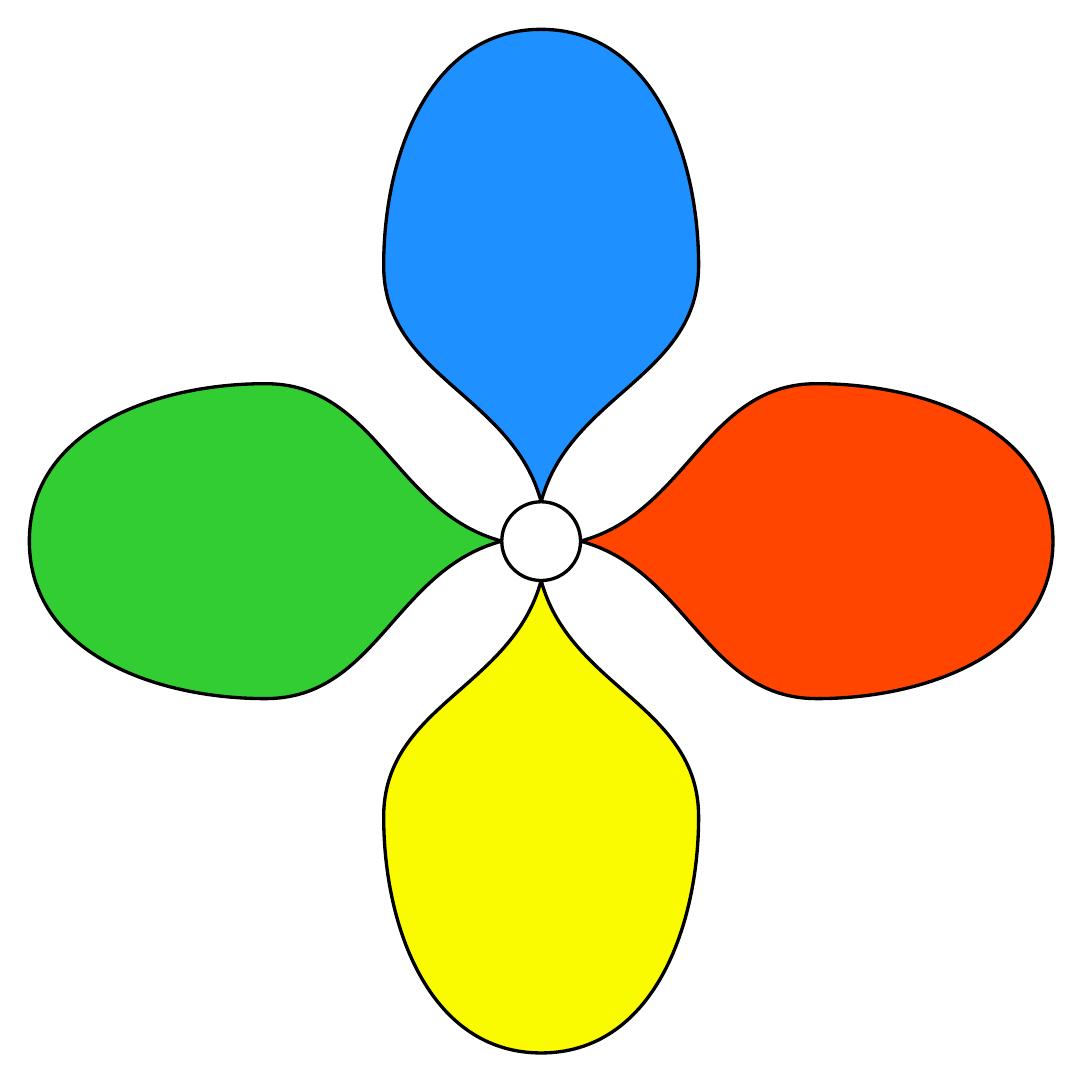
\begin{tikzpicture}[very thick]
\draw[fill=dogerblue] (0,6.5) to[out=0,in=90] 
  ++(2,-3)  to[out=-90,in=75] 
  ++(-2,-3) to[out=105,in=-90] 
  ++(-2,3)  to[out=90,in=180] cycle;
\draw[fill=darkyellow] (0,-6.5) to[out=0,in=-90] 
  ++(2,3)  to[out=90,in=-75] 
  ++(-2,3) to[out=-105,in=90] 
  ++(-2,-3)  to[out=-90,in=180] cycle;
\draw[fill=orangered] (6.5,0) to[out=90,in=0] 
  ++(-3,2)  to[out=180,in=15] 
  ++(-3,-2) to[out=-15,in=180] 
  ++(3,-2)  to[out=0,in=-90] cycle;
\draw[fill=limegreen] (-6.5,0) to[out=90,in=180] 
  ++(3,2)  to[out=0,in=165] 
  ++(3,-2) to[out=195,in=0] 
  ++(-3,-2)  to[out=180,in=-90] cycle;
\draw[fill=white] (0,0) circle (0.5cm);
\end{tikzpicture}

\end{document}